\documentclass[dissertation.tex]{subfiles}
\begin{document}

\chapter{Signatures of Survival Processes in Pancreatic Cancer}
\label{chap:signatures}

\mpfatal{TODO: put the thesis somewhere: That specific molecular processes control survival of resectable PC, and that these processes can be identified and detected using GEX data.}

\section{Introduction}

\paragraph{Summary}Very little is known regarding the biological processes that control the survival of patients with \gls{PDAC}, the most common and aggressive form of pancreas cancer.  As discussed in chapter \ref{chap:nomogram}, the wide range of relative patient survival times that is observed in practice is not well explained by extrinsic factors such as age at diagnosis, and perhaps instead reflects differences in the biological processes operating within each tumour.  Recent molecular profiling work has identified possible molecular subtypes within the previously homogenous group of \gls{PDAC}, but these subtypes have not achieved the maturity or clinical application of those in breast cancer, and their discovery and validation has been hampered by ad-hoc methodology, and the lack of large, well-curated cohorts of \gls{PDAC} samples.  The recently-compiled \gls{APGI} cohort contains the largest group of clinically annotated \gls{PDAC} samples, with accompanying \gls{GEX} and high-quality follow-up data, in the world.  It presents a unique opportunity to apply modern techniques for prognostic signature identification to the discovery of biological processes that drive the clinical course of pancreas cancer.  These signatures may find application as prognostic tools in their own right, but more importantly can supply much-needed information on the fundamental biology of the one common cancer that has, to date, been almost entirely refractory to all the tools of modern molecular medicine.

\vspace{1cm}

Despite extensive research, \gls{PDAC} remains a poorly-understood disease.  Recent genomic profiling has revealed the genetic alterations that accompany the disease \cite{Biankin2012}, and a staggering number of prognostic factors are known \cite{Harsha2009}, but these findings have shed little light on the fundamental disease processes at work in individual tumours.  This is a consequence of genetic and biomarker data being poorly-suited for understanding the biological state of a cell: although genetic alterations are central to the etiology of cancer, they give incomplete information on the pathways and systems actually active in a given tumour, and biomarkers represent non-causal readouts of cell state that are difficult to trace back to underlying biological processes.

Sitting between the regulatory function of transcription control, and the effector function of protein expression, \gls{GEX} data integrate information from all aspects of cell condition, including genetic alterations, signalling pathway activity, and metabolic status.  As such, it is unsurprising that \gls{GEX} data are superior indicators of cell state, better than all other high-throughput measurement methods, such as protein expression or genetic alterations \cite{Ray2014}.  However, the involvement of \gls{GEX} with so many biological inputs is also a weakness: typical differential expression studies will identify many hundreds of transcripts that vary between disease states, and the deconvolution of this complex set of hundreds of effects back to a small number of causative molecular processes remains challenging.

Historically, disease \gls{GEX} profiling studies have largely refrained from attempting to infer the state of a few molecular processes from the many hundreds of differentially-expressed genes identified; notable early exceptions are for example \mpfatal{PCA, ICA cites}.  A number of factors are likely to have contributed to this reluctance: deconvolution methods are numerically sensitive and require very large sets of high-quality measurements, early techniques were poorly-suited to the particular requirements of the \gls{GEX} deconvolution problem, and the signature databases that assist the assignation of a biological annotation to the output from a deconvolution calculation (for example, the \acrshort{MSigDB} \cite{Subramanian2005}) have only recently reached maturity.

In addition to the general technical challenges of \gls{GEX} deconvolution, issues particular to pancreas cancer significantly complicate attempts to identify molecular processes at work within the tumours.  Pancreas cancer is challenging to sample, and mRNA in the tissue degrades rapidly once extracted, complicating sample collection.  Additionally, a feature of \gls{PDAC} is the presence of a dense desmoplastic stromal reaction throughout the tumour, that is formed by genetically normal patient stroma cells \cite{Mahadevan2007}.  The fraction of tumour cells that are stromal varies by more than 10-fold between tumours \cite{Biankin2012}, meaning that without careful correction, gene expression profiles are dominated by stromal cell fraction signals, and not true differential expression within a cell type.  Microdissection has been used to separate cancer cells from surrounding stroma in order to simplify analysis \cite{Collisson2011}, but current thought in the field is that the stroma in \gls{PDAC} is an essential and enabling, if not in itself neoplastic, component of the tumour \cite{Mahadevan2007}, and that the examination of cancer cell expression in isolation ignores the likely important interplay between the two major synergistic components of a tumour: transformed epithelial cells, and genetically normal stroma.

Due to these challenges to \gls{GEX} deconvolution of \gls{PDAC}, to date only one study (by Collisson et al) has reported a breakdown of \gls{PDAC} \gls{GEX} into a small number of biological modules \cite{Collisson2011}.  This study examined microdissected cancer cells only, and found that the transformed epithelial cells of \gls{PDAC} could be placed into three major categories, based on their patterns of gene expression.  Tumours from these three categories followed distinct clinical courses, and cell lines exhibited category-specific sensitivity to therapeutic drugs.  As the first report to identify potential clinically relevant molecular subtypes within \gls{PDAC}, the Collisson study was a significant advance in the understanding of the molecular processes at play within what was previously considered a homogeneous disease.  However, it also possesses some failings that reduce its clinical utility.

Two main issues complicate the interpretation of the Collisson classes: microdissected cancer cells were used, and therefore stromal effects would be severely attenuated; and the deconvolution technique employed was tuned to achieve sample clustering, rather than \gls{GEX} deconvolution.  Consequently, although the Collisson classes could be a fundamental advance in the understanding of \gls{PDAC}, they necessarily do not consider the full context of the disease, and potentially have artifically identified subgroups when in reality a smooth continuum of disease types may exist.  Additionally, although the Collisson subgroups display a link with clinical course, they were not explicitly generated for this purpose.

A substantial gap remains in our molecular understanding of \gls{PDAC}: nothing is known about the core molecular processes at work within both the cancer and stroma of different tumours, and particularly those processes that may control patient survival following diagnosis.  Such a gap in knowledge is not merely of academic interest: a better understanding of the processes affecting patient survival can lead directly to improved methods for staging, and ultimately may stratify patients for customised therapies, and even suggest targets for therapeutics capable of transforming a poor-prognosis cancer into a good-prognosis one.  The primary obstacle for the identification of these survival-associated processes in \gls{PDAC} is one of data: a large, high-quality dataset of \gls{GEX} measurements and associated well-curated \glspl{CPV} is needed.  The \gls{APGI} cohort addresses this data problem for the identification of fundamental survival processes in \gls{PDAC}.  As the largest cohort of \gls{PDAC} samples, with accompanying \gls{GEX} and curated \glspl{CPV}, in the world, it can provide the data quality and cohort size required by modern \gls{GEX} deconvolution techniques.

In this chapter I describe the application of \gls{NMF} for the \gls{GEX} deconvolution of genes associated with outcome.  The metagenes thus identified represent orthogonal coordinately-expressed sets of genes which I then map to biological annotations, identifying the fundamental processes that may be involved in controlling the clinical course of a patient's pancreas cancer.  The results of this work are directly applicable as signatures of survival time following diagnosis of \gls{PDAC}, and also identify discrete biological processes that appear to determine outcome with pancreas cancer, and represent fertile future avenues for research into this poorly-understood disease.


\section{Results}

Survival-associated metagenes were identified by selecting the set of genes which had \gls{GEX} associated with outcome in the \gls{APGI} cohort, and then performing \gls{NMF} factorization to deconvolve the full matrix of gene expression signals into a small set of metagenes.  Metagenes were then tested for association with clinical course and other \glspl{CPV}, as well as known prognostic signatures, and their prognostic ability was validated by 10-fold cross-validation and testing in separate cohorts.  Those metagenes that were found to be prognostic were then correlated with biological process signatures to associate the metagenes with biological processes.

\subsection{Cohort characteristics and subsetting}
The same homogeneous \gls{PDAC} subset of the \gls{APGI} cohort that was used in the work of chapter \ref{chap:nomogram} was employed for this analysis; see page \pageref{chap:nomogram} for case selection criteria and cohort characteristics.  \mpfatal{Add correct ref label}

\subsection{Two metagenes predict survival with resectable pancreatic cancer in multiple cohorts}
\paragraph{Probe selection}
In order to focus the \gls{GEX} deconvolution method on finding outcome-associated metagenes, it was necessary to filter the full set of gene expression data to only contain those genes that were likely to be associated with patient survival.  %This has traditionally been considered to be a very difficult problem, due to the huge number of candidate genes present and the relatively small number of patients available.

%However, recent results in variable selection theory have indicated that marginal screening procedures are sufficient for variable selection \cite{Fan2008}, including in censored regression situations (for example \cite{Gorst-Rasmussen2013}).  Unfortunately, although most of these procedures guarantee good variable selection properties in general, a specific issue remains: it is unknown exactly \emph{how many} variables need to be chosen in order to achieve a given false rejection or false discovery rate.  This is equivalent to the problem of deciding a selection threshold for the procedures, and the difficulty in choosing such a threshold is a serious impediment to the practical application of these methods.

%The emerging field of stability selection has provided some solutions to the practical issue with the marginal screening methods described above.  The concept is simple: repeat the genes selection method multiple times on perturbed variants of the original data, and select only those genes that are consistently chosen.  Recent work has produced the \gls{CPSS} algorithm, which provides bounds on the false detection rate of the variable selection procedure \cite{Shah2013}.

A \gls{CPSS} wrapper around the core \gls{SIS}-\gls{FAST} variable selection method \cite{Gorst-Rasmussen2013} identified 193 genes (of 13,000 considered) that were associated with time from diagnosis to disease-specific death in the \gls{APGI} cohort, with an estimated \gls{FDR} of approximately 5\%.

\paragraph{Factorization}
%Central to the concept of \gls{GEX} deconvolution is the idea that the observed expression of a given gene in a sample is the sum of that gene's expression due to each of the biological processes operating in the cell.  By examining enough sufficiently diverse samples, it is hoped to estimate three elements: the number of basic processes at work in the cells, the level of activity of each process within each sample, and the degree to which the activity of a process increases the expression of a gene.  More concretely, let the concentration of a gene's transcripts be denoted by $a$, in arbitrary linear units, such as copies per cell.  Suppose that $r$ basic biological processes are operating in the cell, and that these are numbered $1, 2, \dots, r$.  Each process can have a level of activation ranging from zero to one, where zero is off, and one is completely on.  Also, the activation of each process can affect the concentration of the gene's transcripts to a different degree: activation of one process may lead to strong expression of the gene, whereas the level of activation of another process may have no influence on the gene's transcript levels at all.  Let the level of activation of process $i$ be $h_i$, and the influence of process $i$ on the expression levels of the gene be $w_i$.  Then, the basic model underpinning this work is:
%\begin{equation}
%  a = h_1 w_1 + h_2 w_2 + \dots + h_r w_r = \sum_{i=1}^r h_i w_i
%\end{equation}
%In words, the expression of a transcript is the sum of the level of activation of each process in the cell on that transcript, weighted by the activity of that process in the sample.

%For convenience, in the explanation above I have termed the $r$ processes that are active in each cell `biological processes'.  This is a simplification.  These components are generally termed `metagenes' in the factorization literature, and I will use this term predominantly from this point onwards.  Metagenes represent sets of genes that are closely coordinately transcribed, and therefore can, in a sense, be considered to act transcriptionally like a single unit.  Metagenes do not necessarily have to equate to what would more conventionally be considered to be `biological processes', such as cell motility or metabolism, but as likely targets of the same set of transcription factors, often do correlate with discrete aspects of cell function.

%It is straightforward to extend the model above to the more general case of multiple transcripts and multiple samples; the equation now becomes
%\begin{equation}
%  A = W H
%\end{equation}
%Here $A$ is a transcript $\times$ sample matrix of linear gene expression measurements, $W$ is a transcript $\times$ metagene activation matrix (termed the \emph{basis} matrix in the subject literature), and $H$ is a metagene $\times$ sample activity matrix (the \emph{coefficient} matrix in the literature).  Expression deconvolution now becomes a matrix factorization problem, for which a wide range of techniques are available.

The expression of the 193 survival-associated genes across 228 patients was decomposed into metagenes by the \gls{SNMFL} \gls{NMF} algorithm.  The number of metagenes (factorization rank) was automatically estimated to be 6, being the lowest rank for which the improvement in estimation error achieved by adding the next rank, was less than that observed for permuted data (figure \ref{fig:sig_nmf_rank}).

\begin{figure}
\centering
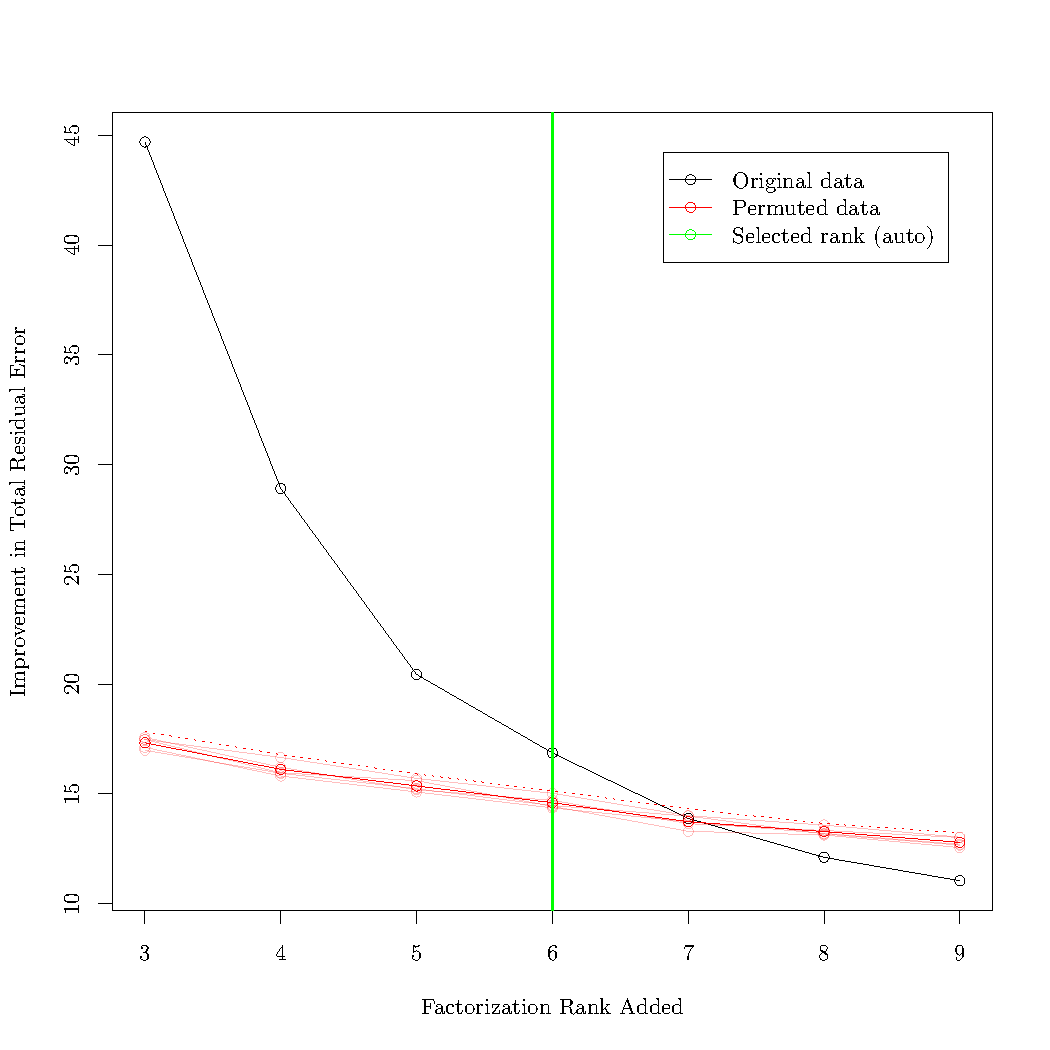
\includegraphics[width=.7\linewidth]{analysis/biosurv/reports/18_SIS_diag_dsd_final/figure/nmf-rank-plots-2}
\caption{Automatic selection of factorization rank.  \acrshort{SNMFL} was performed for varying ranks on either unpermuted data (black line) or data permuted within samples (red lines), and the improvement in total residual approximation error $\|A - W H\|_2$ calculated.  The highest added rank for which the error improvement on unpermuted data exceeded that of permuted data plus two standard deviations (threshold shown by dotted red line) was the final selected rank (green line).}
\label{fig:sig_nmf_rank}
\end{figure}

500 random restarts of rank 6 \gls{SNMFL} were then performed on the survival-associated gene matrix to yield the final factorization.  The resultant clustering consensus matrix was highly stable (figure \ref{fig:sig_nmf_consensus}), and the basis matrix $W$ was reasonably sparse (figure \ref{fig:sig_nmf_basis}).  Small row L1 norm of the basis matrix is a desirable condition for this analysis, as it indicates that metagenes are largely distinct transcriptional modules, with little overlap in terms of shared transcripts with high loadings; \gls{SNMFL} was selected for its penalty design, which favours solutions with small $W$ row L1 norm.  A table of values of the basis matrix $W$ is available as appendix \ref{app:sig_w_matrix} on page \pageref{app:sig_w_matrix}}

\begin{figure}
\centering
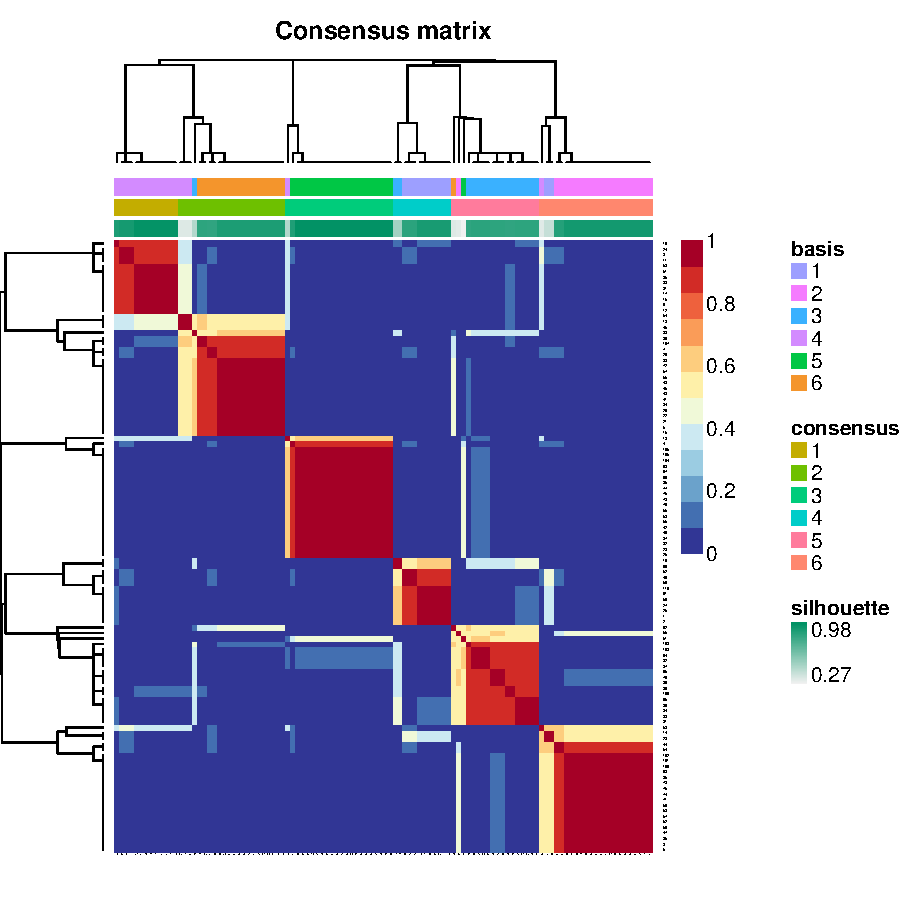
\includegraphics[width=.7\linewidth]{analysis/biosurv/reports/18_SIS_diag_dsd_final/figure/nmf-plots-1}
\caption{Clustering consensus matrix for the final rank-6 clustering.  Colours indicate the stability of gene (in rows) and sample (in columns) clusters across random restarts of the factorization; at rank 6 this factorization was perfectly stable, with identical clusters observed in all 500 random restarts.}
\label{fig:sig_nmf_consensus}
\end{figure}

\begin{figure}
\centering
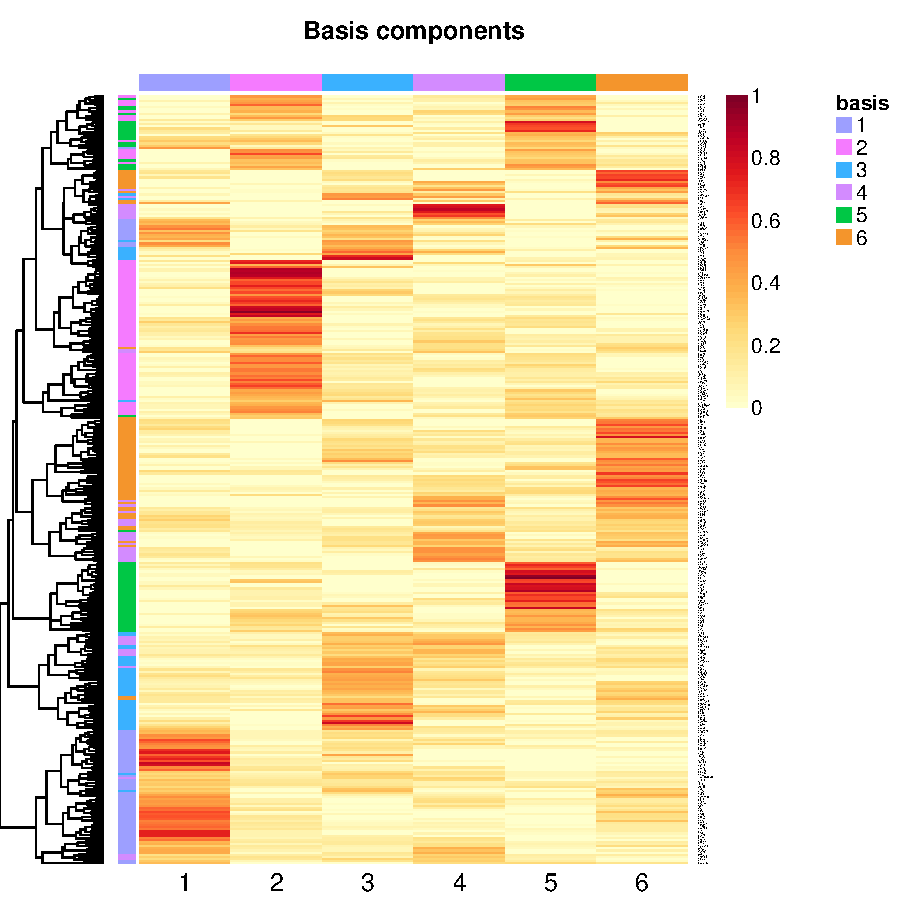
\includegraphics[width=.7\linewidth]{analysis/biosurv/reports/18_SIS_diag_dsd_final/figure/nmf-plots-2}
\label{fig:sig_nmf_basis}
\caption{Basis matrix of the final \acrshort{SNMFL} factorization.  Rows represent genes, and columns metagenes, with cell colours proportional to the loading of a given gene on a given metagene.  The loadings are sparse within rows, indicating that the metagenes are modular, each affecting the expression of largely distinct sets of target genes.  A table of values of this basis matrix is available as appendix \ref{app:sig_w_matrix} on page \pageref{app:sig_w_matrix}}
\end{figure}

\paragraph{Identifying prognostic metagenes}
The transcription patterns of genes associated with survival in the \gls{APGI} cohort could be decomposed into just six largely distinct metagenes.  To identify which of the six metagenes were ultimately predictive of patient survival, I performed \gls{LASSO} regression on the \gls{APGI} discovery cohort data, using \gls{NNLS}-estimated coefficients of each of the six metagenes as marginal predictors of outcome.  The \gls{LASSO} regularization parameter $\lambda$ was chosen by 10-fold cross-validation to be the highest value for which the mean test set partial likelihood deviance was within one standard error of the lowest mean value.  This resulted in a final model in which only two metagenes, MG3 and MG6, were selected as prognostic (figure \ref{fig:sig_resub_lasso_track}).

\begin{figure}
\centering
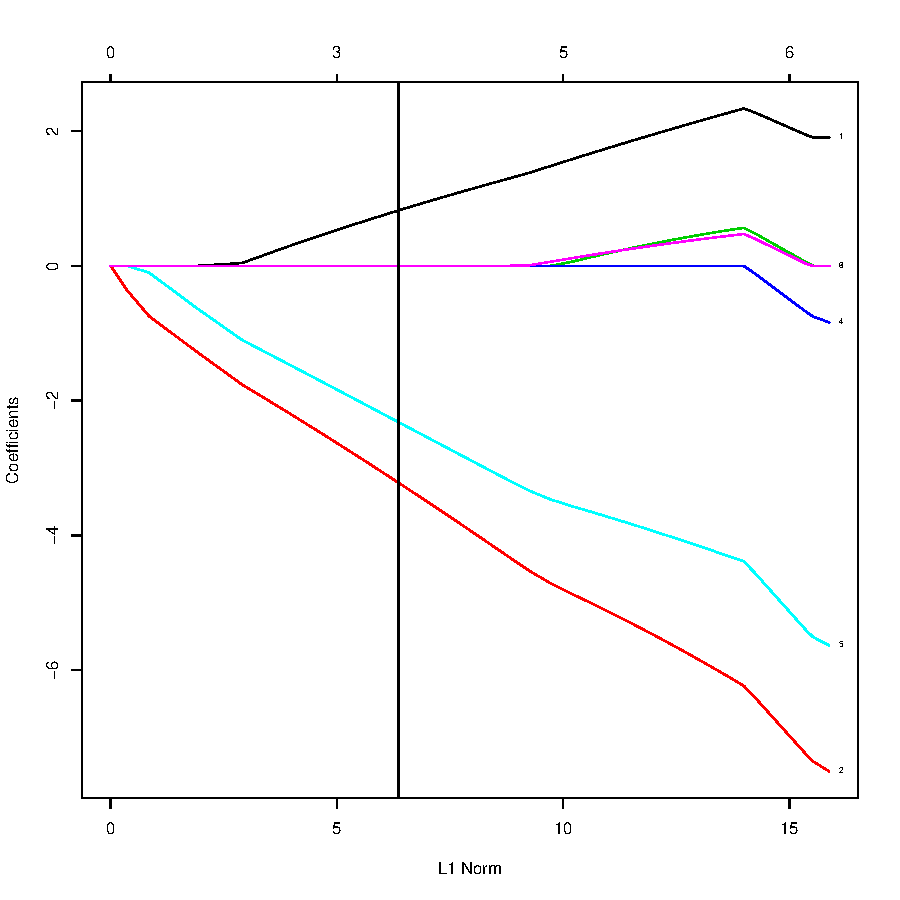
\includegraphics[width=.7\linewidth]{analysis/biosurv/reports/18_SIS_diag_dsd_final/figure/nmf-metagene-glmnet-plots-2}
\label{fig:sig_resub_lasso_track}
\caption{Coefficient vs penalty fit trajectories for the \acrshort{LASSO} model predicting disease-specific survival from metagene expression.  Each coloured line represents the model coefficient for a metagene as the model is smoothly varied from a null model (L1 norm = 0), to a full unpenalised Cox fit (L1 norm $\approx$ 14).  The vertical line indicates the optimal value of L1 norm as selected by 10-fold cross-validation; at this point in the trajectory only metagenes MG3 and MG6 make any contribution to prognosis estimates.}
\end{figure}

The final signature developed for predicting time from diagnosis to death for patients \gls{PDAC} therefore consists of distinct two metagenes: the protective MG3, and the hazardous MG6.  For external validation of the signature I combined observed coefficients for the two metagenes using their CV-selected \gls{LASSO} fit coefficients, as $\text{Risk score} = -0.4086 \times \text{MG3 coefficient} + 3.3022 \times \text{MG6 coefficient}$.  Full metagene scores for the 193 survival-associated genes (the $W$ matrix) are available as appendix \ref{app:sig_w_matrix} on page \pageref{app:sig_w_matrix}. \mpfatal{Put these scores in}

\paragraph{Validation of the two-metagene signature}
To ensure that the process for development of the two-metagene survival signature was stable, and that the signature itself was transferable to other cohorts, I performed cross- and external validation of the metagene survival signature.  10-fold cross-validation was performed on the full metagene discovery procedure, from supervised probe selection by \gls{CPSS}-\gls{SIS}-\gls{FAST} to final \gls{LASSO} coefficient estimation, including automatic \gls{NMF} rank estimation.  Cross-validated test set risk scores from the \gls{APGI} discovery cohort were significantly predictive of time from diagnosis to disease-specific death by Cox regression (LRT $P = 0.0029$).  The two-metagene survival signature described above also validated against the \gls{PDAC} expression cohort GSE28735 \cite{Zhang2013} (LRT $P = 0.0171$), demonstrating the robustness of the metagene signature to cohort and platform effects.

\subsection{Prognostic metagenes implicate the \acrshort{EMT} and MYB in pancreatic cancer outcome}

\section{Discussion}

\section{Methods}
\subsection{Cohort recruitment and ethics}
\mpfatal{CPVs current as of 4 Nov 2014}

\subsection{Sample collection, preparation, and gene expression microarrays}
\mpfatal{}
End with saved as \gls{IDAT} files.  241 of them (class 7 with CPVs only)

\subsection{Data preprocessing}
\paragraph{Microarray quality control and normalization}
\gls{IDAT} files were read into Bioconductor \texttt{lumi} structures using the \texttt{lumidat} package.  Seven arrays were excluded on the basis of poor signal, due to fewer than 30\% of probes on these arrays having detection P-values of less than 0.01.  The remaining 234 microarrays represented a range of tumour types, and were normalized as one batch using the \texttt{lumi} package.  Normalization proceeded serially as: RMA-like background subtraction (\texttt{lumiB} method \texttt{"bgAdjust.affy"}), \gls{VST} (\texttt{lumiT} method \texttt{"vst"}), and quantile normalization (\texttt{lumiN} method \texttt{"quantile"}).

\paragraph{Unsupervised probe selection}
Probes were excluded if they met any of the following criteria: fewer than 10\% of samples with expression P-values of less than 0.01, a probe quality (from the \texttt{illuminaHumanv4PROBEQUALITY} field in Bioconductor package \texttt{illuminaHumanv4.db}) not equal to `perfect' or `good', missing gene annotation, or a standard deviation of normalized expression values across all samples of less than 0.03.  The choice of this latter threshold is expected to yield approximately a 5\% false probe rejection rate, based on an analysis of the variation between technical replicate samples.  In cases where multiple post-filter microarray probes mapped to the same gene, only the probe with the highest standard deviation, as evaluated across all samples that passed quality checks, was retained.  The effect of these combined filtering steps was to reduce the number of features under consideration from 47,273 probes to 13,000, one per gene.

\paragraph{Sample selection}  From the full set of 234 tumour samples that passed quality checks, eight were from four samples that had each been arrayed twice, and two were from patients with multiple conflicting \gls{CPV} data.  The two with conflicting \gls{CPV} data were excluded from further study, and the eight replicated samples were averaged, after \gls{MDS} indicated that each replicate pair had very similar expression.

\paragraph{Summary}
The above preprocessing steps yielded matched \gls{CPV} and resected tumour \gls{GEX} data for 13,000 genes across 228 patients.

\subsection{Outcome-associated gene selection}
Genes that were associated with disease-specific survival were identified by \gls{SIS}-\gls{FAST} \cite{Gorst-Rasmussen2013}, with a \gls{CPSS} wrapper to reduce the false positive rate \cite{Shah2013}.  The inner \gls{SIS}-\gls{FAST} selectors from R package \texttt{ahaz} each provided 650 genes associated with time between diagnosis and death, and the outer \gls{CPSS} wrapper selected genes which were returned by at least 75\% of \gls{SIS}-\gls{FAST} runs.  193 genes passed this criterion and were selected for closer study.  
In the terminology of \cite{Shah2013}, the parameters of this selection procedure were $\theta = 0.05$, $\tau = 0.72$, and therefore the expected bound on the number of false positive genes in the set of 193 was ten \cite[table 1]{Shah2013}, yielding a gene \gls{FDR} of approximately 0.05.

\subsection{Rank estimation and metagene factorization}
\label{subsec:signatures-nmf}
The gene $\times$ patient expression matrix of outcome-associated genes was decomposed into metagenes by the \gls{SNMFL} procedure of \cite{Kim2007}, as implemented in R package \texttt{NMF}.  \gls{SNMFL} is a variant of \gls{NMF}, a class of procedures that decomposes a non-negative matrix $A$ into a product of non-negative matrices $W$ and $H$, $A \approx WH$.  $W$ and $H$ typically have rank much less than $A$, the effect of \gls{NMF} then being to effectively reduce a large gene $\times$ sample matrix $A$ into smaller matrices, the gene $\times$ metagene basis matrix $W$, and metagene $\times$ sample coefficient matrix $H$.

As \gls{NMF} is a linear factorization, the \gls{VST}-transformed expression matrix $A$ was approximately linearized by elementwise exponentiation, $a_{i,j} \leftarrow 2^{a_{i,j}}$.  To reduce the influence of large variations in baseline expression on the factorization, each row (gene) of $A$ was then independently linearly scaled to lie between zero and one, $a_{i,j} \leftarrow (a_{i,j} - \min(a_{i,*})) \div (\max(a_{i,*}) - \min(a_{i,*}))$, where $a_{i,*}$ denotes row $i$ of $A$.

Factorization rank was estimated following \cite{Frigyesi2008}: for test ranks ranging from 2 to 15, 10 \gls{SNMFL} decompositions were performed, each on a version of the transformed expression matrix in which rows (genes) had been independently permuted within each column (sample).  Approximation error for each decomposition was calculated as $\|A - W H\|_F$, and the reduction in approximation error with increasing rank was compared between factorizations of the original data, and those of the 10 permuted data matrices.  The highest rank for which the improvement in error achieved by adding that rank to the factorization on the original data, exceeded the improvement seen by adding that rank on the permuted data, taking into account permutation noise, was selected as the final factorization rank.  Specifically, let the improvement in approximation error that results in choosing a rank $i$ decomposition over a rank $i-1$ decomposition, on the unpermuted data, be $\Delta_i = \|A - W_{i-1} H_{i-1}\|_F - \|A - W_{i} H_{i}\|_F$.  Equivalently, define $\Delta^{*j}_i$ to be the improvement observed when rank $i$ is added to the factorization of $A^{*j}$, the $j$\textsuperscript{th} permutation of the data matrix: $\Delta^{*j}_i = \|A^{*j} - W^{*j}_{i-1} H^{*j}_{i-1}\|_F - \|A^{*j} - W^{*j}_{i} H^{*j}_{i}\|_F$.  Denote the mean and standard deviation of $\Delta^{*}_i$ across all 10 permutations of the data matrix, for each $i$, as $\overline{\Delta^{*}_i}$ and $\text{SD}(\Delta^{*}_i)$, respectively.  Then, the final selected rank $k$ was identified as $k = \argmax_i \Delta_i > \overline{\Delta^{*}_i} + 2 \text{SD}(\Delta^{*}_i)$.

Following rank estimation, a final factorization of the data was performed using only the identified rank, and a larger number of random algorithm restarts, as described below.  Subsequent work used this final factorization.

The \gls{SNMFL} algorithm requires parameters $\alpha$ and $\eta$ to control regularization; for all factorizations $\alpha = 0.01$, and $\eta = \max(A)$.\footnote{Note that this parameter $\alpha$ is denoted $\beta$ in the R \texttt{NMF} package; I use the symbol $\alpha$ here for consistency with \cite{Kim2007}}  The default convergence criteria of by the \texttt{NMF} package were used.

\gls{SNMFL} may not necessarily find a global optimum factorization; for this work multiple random initializations of matrix $W$ were made from $\text{Uniform}(0, \max(A))$, the \gls{SNMFL} procedure was run to convergence, and the result with lowest approximation error was retained.  50 random restarts were used during rank estimation runs, and 500 for the final factorization; examination of approximation error distributions for these repeated runs indicated that these values were conservative, and factorizations were very robust to the choice of random start.

\subsection{Estimating metagene coefficients on new data}
The following procedure was used to estimate metagene expression scores (coefficients) from gene expression measurements of a cohort.  Measurements were subset to the 193 outcome-associated genes identified by \gls{CPSS}-\gls{SIS}-\gls{FAST}, and transformed to a linear scale if necessary.  Linear measurements were then scaled within genes to between zero and one, as for metagene factorization (section \ref{subsec:signatures-nmf}).  Genes for which no expression data were available (the genes being either filtered out in preprocessing or not measured at all) were assigned scaled expression values of zero.  These manipulations yielded a gene $\times$ sample matrix $A'$ with rows matching the gene $\times$ metagene basis matrix $W$ from \gls{SNMFL}.  The metagene $\times$ sample coefficient matrix $H'$ for the new cohort was then estimated by \gls{NNLS} implemented in R package \texttt{nnls}, solving for each column of $a'_{*,i}$ of $A'$ the optimization problem ${h'_{*,i}} = \argmin_x \| W x - a'_{*,i} \|_2$, where $h'_{*,i}$ denotes column $i$ of $H'$.

For consistency, the above procedure was used to estimate metagene coefficients $H$ for the discovery \gls{APGI} cohort, as well as all validation cohorts.

\subsection{Associating metagene expression with clinical variables}

\subsection{Cross-validation of the metagene discovery process}

\subsection{External validation of outcome-associated metagenes}

\subsection{\acrshort{GSVA} scoring}
The expression of gene sets from the \gls{MSigDB} \cite{Subramanian2005} were estimated on the \gls{APGI} cohort using a modification of the \gls{GSVA} method \cite{Hanzelmann2013}.  \gls{GSVA} with default settings was used to estimate expression scores for all \gls{MSigDB} gene sets in the full 13,000 $\times$ 228 \gls{VST}-scaled \gls{APGI} \gls{GEX} data matrix.  \gls{MSigDB} contains both undirected gene sets such as metabolic pathways, in which members of the set are not expected a-priori to move in concert, and directional signatures, with paired \texttt{*\_UP} and \texttt{*\_DN} components that would be expected to change in coordinated and opposite patterns.  Conventional analyses based on \gls{MSigDB} ignore this distinction, but for this work I combined paired directional signatures to yield an overall signed estimate of signature activity.  For undirected signatures, \gls{GSVA} activity estimates were simply calculated using parameter \texttt{abs.ranking=TRUE}.  In the case of paired signatures, \gls{GSVA} scores were estimated separately for the \texttt{*\_UP} and \texttt{*\_DN} sets using parameter \texttt{abs.ranking=FALSE}, and the signed combined activity \texttt{*\_SIGNED} was calculated as the \texttt{*\_DN} score subtracted from the \texttt{*\_UP} score.  This procedure resulted in summarised activity estimates for 8,138 gene sets, many of which were highly correlated.

Gene sets with highly correlated activity scores were collapsed into compound summary sets as follows.  Pairwise Pearson correlation distances between all scores calculated as $d_{i,j} = \frac{1}{2}(1 - \text{cor}(s_i, s_j))$, and were used to cluster gene sets using R \texttt{hclust} and complete linkage.  R \texttt{cutree} identified clusters of highly similar gene sets, using a distance threshold of 0.02; gene set activities within each cluster were merged by taking median values across all samples, to form a new merged gene set activity estimate.  Following merging, 7,633 single and compound gene set activity estimates remained across 228 samples.

\subsection{Metagene functional characterization}
Kendall correlation coefficients were calculated between metagene coefficients and \gls{GSVA} gene set scores, on the \gls{APGI} expression dataset.  Absolute correlations of greater than 0.5 were deemed substantive and reported for further characterisation.


\end{document}
